\chapter{User Manual}
This chapter provides an explanation of the canvas and how to manipulate the tools provided. Below is what a blank canvas will look like:
\begin{figure}[h!]
\centering
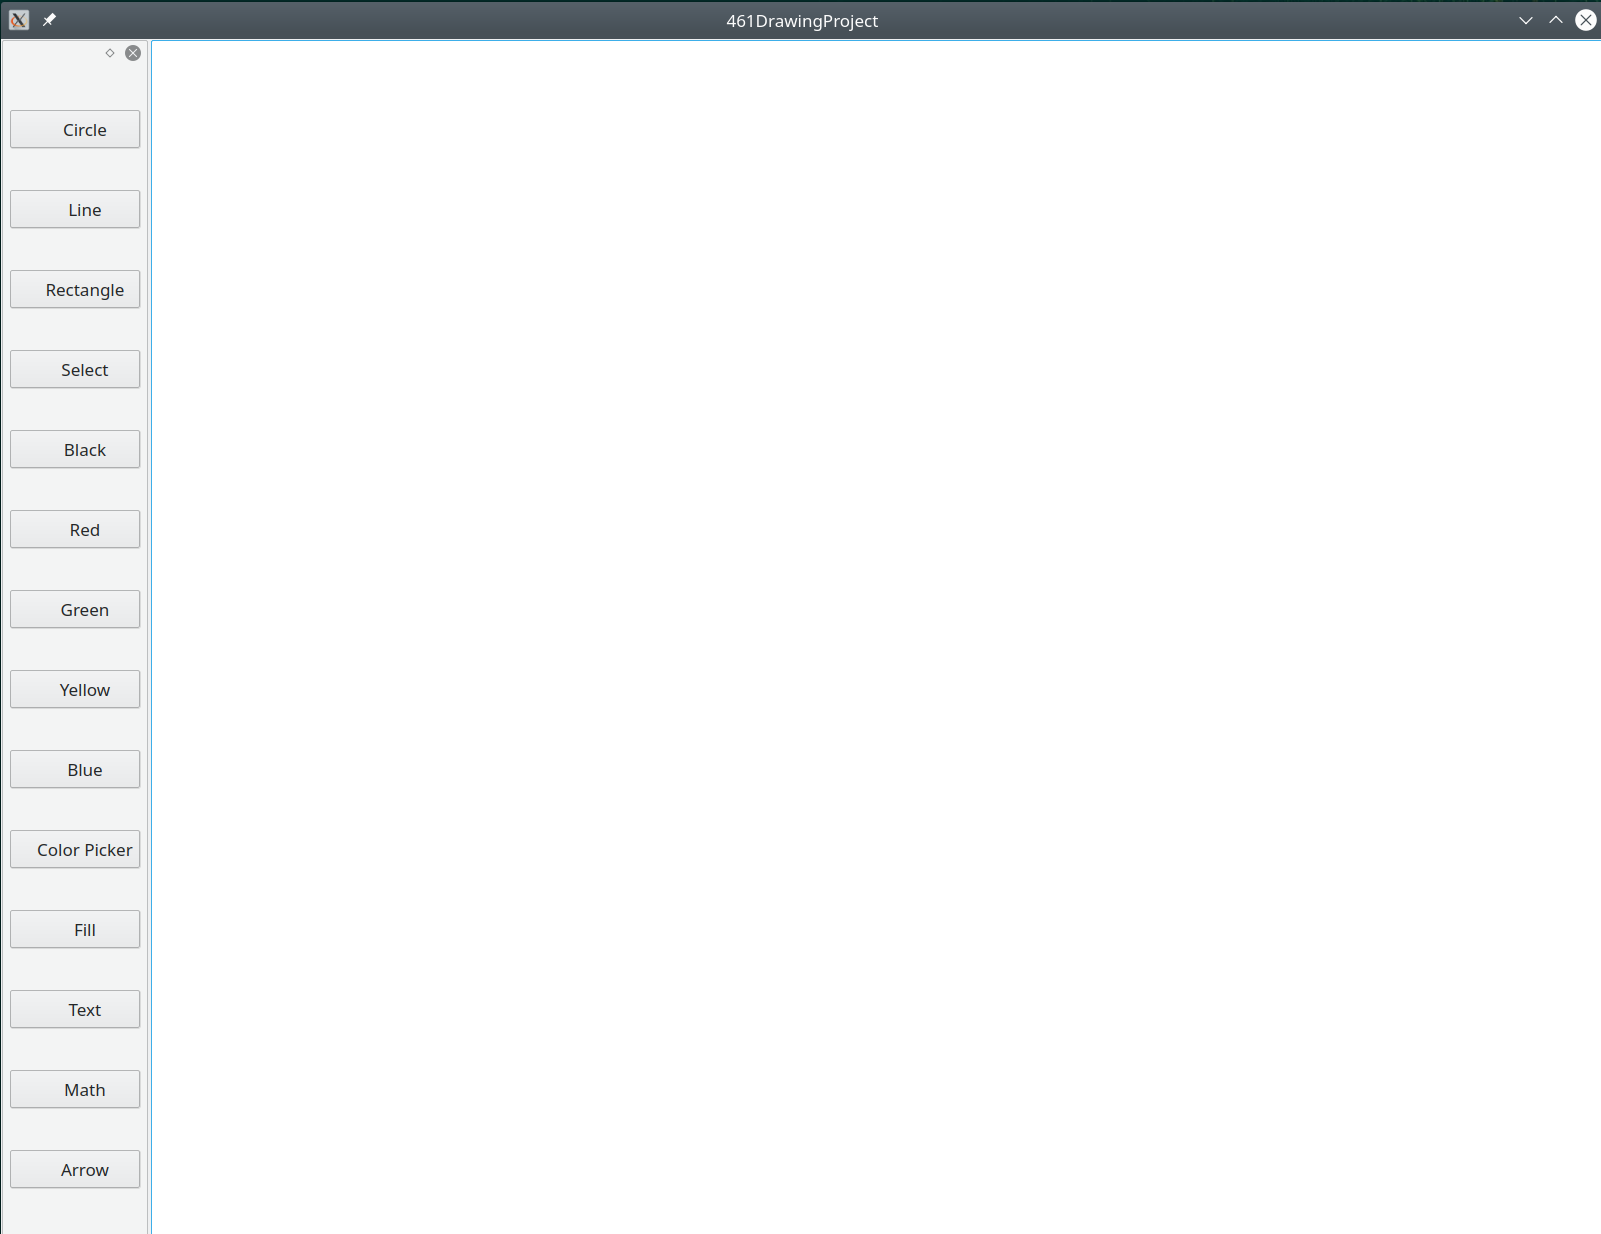
\includegraphics[height=10cm, width=10cm]{canvas}
\caption{Blank Canvas}
\end{figure}

\section{Manipulating Items}
\subsection{Select}
\begin{figure}[h!]

\includegraphics{select}
\end{figure}
  The way to manipulate items drawn on the canvas is to use the "select" tool. With the select tool equipped click, hold, and drag an item to the desired location, then release the item and it will be relocated to its new position.


\section{Drawing}
Below is an explanation on how to use each drawing tool

\subsection{Lines}
\begin{figure}[h!]

\includegraphics{line}
\end{figure}
Select the line button, then on the canvas, click two separate points you want to draw a line between.

\subsection{Rectangles}
\begin{figure}[h!]

\includegraphics{rect}
\end{figure}
Select the rectangle button, then on the canvas, click one point to be the top right corner and click the second point to be the bottom left corner and a rectangle will be drawn in between.

\subsection{Circle}
\begin{figure}[h!]

\includegraphics{circle}
\end{figure}
Select the Circle button, then on the canvas, click two separate points, the first is the center point and the second is the radius. A circle will be drawn using those two reference points.

\subsection{Arrow}
\begin{figure}[h!]

\includegraphics{arrow}
\end{figure}
here will be arrow details

\subsection{LaTeX}
\begin{figure}[h!]

\includegraphics{math}
\end{figure}
Select the Math button, then in the text box type in your desired LaTeX code and click the enter button.

\subsection{Text}
\begin{figure}[h!]

\includegraphics{text}
\end{figure}
Select the text button, then in the text box type in your desired sentence and click the enter button.

\subsection{Changing Colors}
\begin{figure}[h!]

\includegraphics{cp}
\end{figure}
There are two ways to change color of the shapes, the first is to select one the colors on the side bar, the second is to click 'Color Picker' and choose a color based on RGB value.

\subsection{Fill}
\begin{figure}[h!]

\includegraphics{fill}
\end{figure}
  The fill tool is used to fill a shape with a desired color. To use the tool first click the "fill" button then click the desired fill color, and finally click within the boundaries of the shape you want to fill.
